% Options for packages loaded elsewhere
\PassOptionsToPackage{unicode}{hyperref}
\PassOptionsToPackage{hyphens}{url}
\PassOptionsToPackage{dvipsnames,svgnames,x11names}{xcolor}
%
\documentclass[
  a4paper,
  DIV=11]{scrartcl}

\usepackage{amsmath,amssymb}
\usepackage{iftex}
\ifPDFTeX
  \usepackage[T1]{fontenc}
  \usepackage[utf8]{inputenc}
  \usepackage{textcomp} % provide euro and other symbols
\else % if luatex or xetex
  \usepackage{unicode-math}
  \defaultfontfeatures{Scale=MatchLowercase}
  \defaultfontfeatures[\rmfamily]{Ligatures=TeX,Scale=1}
\fi
\usepackage{lmodern}
\ifPDFTeX\else  
    % xetex/luatex font selection
\fi
% Use upquote if available, for straight quotes in verbatim environments
\IfFileExists{upquote.sty}{\usepackage{upquote}}{}
\IfFileExists{microtype.sty}{% use microtype if available
  \usepackage[]{microtype}
  \UseMicrotypeSet[protrusion]{basicmath} % disable protrusion for tt fonts
}{}
\makeatletter
\@ifundefined{KOMAClassName}{% if non-KOMA class
  \IfFileExists{parskip.sty}{%
    \usepackage{parskip}
  }{% else
    \setlength{\parindent}{0pt}
    \setlength{\parskip}{6pt plus 2pt minus 1pt}}
}{% if KOMA class
  \KOMAoptions{parskip=half}}
\makeatother
\usepackage{xcolor}
\setlength{\emergencystretch}{3em} % prevent overfull lines
\setcounter{secnumdepth}{-\maxdimen} % remove section numbering
% Make \paragraph and \subparagraph free-standing
\ifx\paragraph\undefined\else
  \let\oldparagraph\paragraph
  \renewcommand{\paragraph}[1]{\oldparagraph{#1}\mbox{}}
\fi
\ifx\subparagraph\undefined\else
  \let\oldsubparagraph\subparagraph
  \renewcommand{\subparagraph}[1]{\oldsubparagraph{#1}\mbox{}}
\fi

\usepackage{color}
\usepackage{fancyvrb}
\newcommand{\VerbBar}{|}
\newcommand{\VERB}{\Verb[commandchars=\\\{\}]}
\DefineVerbatimEnvironment{Highlighting}{Verbatim}{commandchars=\\\{\}}
% Add ',fontsize=\small' for more characters per line
\usepackage{framed}
\definecolor{shadecolor}{RGB}{241,243,245}
\newenvironment{Shaded}{\begin{snugshade}}{\end{snugshade}}
\newcommand{\AlertTok}[1]{\textcolor[rgb]{0.68,0.00,0.00}{#1}}
\newcommand{\AnnotationTok}[1]{\textcolor[rgb]{0.37,0.37,0.37}{#1}}
\newcommand{\AttributeTok}[1]{\textcolor[rgb]{0.40,0.45,0.13}{#1}}
\newcommand{\BaseNTok}[1]{\textcolor[rgb]{0.68,0.00,0.00}{#1}}
\newcommand{\BuiltInTok}[1]{\textcolor[rgb]{0.00,0.23,0.31}{#1}}
\newcommand{\CharTok}[1]{\textcolor[rgb]{0.13,0.47,0.30}{#1}}
\newcommand{\CommentTok}[1]{\textcolor[rgb]{0.37,0.37,0.37}{#1}}
\newcommand{\CommentVarTok}[1]{\textcolor[rgb]{0.37,0.37,0.37}{\textit{#1}}}
\newcommand{\ConstantTok}[1]{\textcolor[rgb]{0.56,0.35,0.01}{#1}}
\newcommand{\ControlFlowTok}[1]{\textcolor[rgb]{0.00,0.23,0.31}{#1}}
\newcommand{\DataTypeTok}[1]{\textcolor[rgb]{0.68,0.00,0.00}{#1}}
\newcommand{\DecValTok}[1]{\textcolor[rgb]{0.68,0.00,0.00}{#1}}
\newcommand{\DocumentationTok}[1]{\textcolor[rgb]{0.37,0.37,0.37}{\textit{#1}}}
\newcommand{\ErrorTok}[1]{\textcolor[rgb]{0.68,0.00,0.00}{#1}}
\newcommand{\ExtensionTok}[1]{\textcolor[rgb]{0.00,0.23,0.31}{#1}}
\newcommand{\FloatTok}[1]{\textcolor[rgb]{0.68,0.00,0.00}{#1}}
\newcommand{\FunctionTok}[1]{\textcolor[rgb]{0.28,0.35,0.67}{#1}}
\newcommand{\ImportTok}[1]{\textcolor[rgb]{0.00,0.46,0.62}{#1}}
\newcommand{\InformationTok}[1]{\textcolor[rgb]{0.37,0.37,0.37}{#1}}
\newcommand{\KeywordTok}[1]{\textcolor[rgb]{0.00,0.23,0.31}{#1}}
\newcommand{\NormalTok}[1]{\textcolor[rgb]{0.00,0.23,0.31}{#1}}
\newcommand{\OperatorTok}[1]{\textcolor[rgb]{0.37,0.37,0.37}{#1}}
\newcommand{\OtherTok}[1]{\textcolor[rgb]{0.00,0.23,0.31}{#1}}
\newcommand{\PreprocessorTok}[1]{\textcolor[rgb]{0.68,0.00,0.00}{#1}}
\newcommand{\RegionMarkerTok}[1]{\textcolor[rgb]{0.00,0.23,0.31}{#1}}
\newcommand{\SpecialCharTok}[1]{\textcolor[rgb]{0.37,0.37,0.37}{#1}}
\newcommand{\SpecialStringTok}[1]{\textcolor[rgb]{0.13,0.47,0.30}{#1}}
\newcommand{\StringTok}[1]{\textcolor[rgb]{0.13,0.47,0.30}{#1}}
\newcommand{\VariableTok}[1]{\textcolor[rgb]{0.07,0.07,0.07}{#1}}
\newcommand{\VerbatimStringTok}[1]{\textcolor[rgb]{0.13,0.47,0.30}{#1}}
\newcommand{\WarningTok}[1]{\textcolor[rgb]{0.37,0.37,0.37}{\textit{#1}}}

\providecommand{\tightlist}{%
  \setlength{\itemsep}{0pt}\setlength{\parskip}{0pt}}\usepackage{longtable,booktabs,array}
\usepackage{calc} % for calculating minipage widths
% Correct order of tables after \paragraph or \subparagraph
\usepackage{etoolbox}
\makeatletter
\patchcmd\longtable{\par}{\if@noskipsec\mbox{}\fi\par}{}{}
\makeatother
% Allow footnotes in longtable head/foot
\IfFileExists{footnotehyper.sty}{\usepackage{footnotehyper}}{\usepackage{footnote}}
\makesavenoteenv{longtable}
\usepackage{graphicx}
\makeatletter
\def\maxwidth{\ifdim\Gin@nat@width>\linewidth\linewidth\else\Gin@nat@width\fi}
\def\maxheight{\ifdim\Gin@nat@height>\textheight\textheight\else\Gin@nat@height\fi}
\makeatother
% Scale images if necessary, so that they will not overflow the page
% margins by default, and it is still possible to overwrite the defaults
% using explicit options in \includegraphics[width, height, ...]{}
\setkeys{Gin}{width=\maxwidth,height=\maxheight,keepaspectratio}
% Set default figure placement to htbp
\makeatletter
\def\fps@figure{htbp}
\makeatother

\KOMAoption{captions}{tableheading}
\makeatletter
\makeatother
\makeatletter
\makeatother
\makeatletter
\@ifpackageloaded{caption}{}{\usepackage{caption}}
\AtBeginDocument{%
\ifdefined\contentsname
  \renewcommand*\contentsname{Inhaltsverzeichnis}
\else
  \newcommand\contentsname{Inhaltsverzeichnis}
\fi
\ifdefined\listfigurename
  \renewcommand*\listfigurename{Abbildungsverzeichnis}
\else
  \newcommand\listfigurename{Abbildungsverzeichnis}
\fi
\ifdefined\listtablename
  \renewcommand*\listtablename{Tabellenverzeichnis}
\else
  \newcommand\listtablename{Tabellenverzeichnis}
\fi
\ifdefined\figurename
  \renewcommand*\figurename{Abbildung}
\else
  \newcommand\figurename{Abbildung}
\fi
\ifdefined\tablename
  \renewcommand*\tablename{Tabelle}
\else
  \newcommand\tablename{Tabelle}
\fi
}
\@ifpackageloaded{float}{}{\usepackage{float}}
\floatstyle{ruled}
\@ifundefined{c@chapter}{\newfloat{codelisting}{h}{lop}}{\newfloat{codelisting}{h}{lop}[chapter]}
\floatname{codelisting}{Listing}
\newcommand*\listoflistings{\listof{codelisting}{Listingverzeichnis}}
\makeatother
\makeatletter
\@ifpackageloaded{caption}{}{\usepackage{caption}}
\@ifpackageloaded{subcaption}{}{\usepackage{subcaption}}
\makeatother
\makeatletter
\@ifpackageloaded{tcolorbox}{}{\usepackage[skins,breakable]{tcolorbox}}
\makeatother
\makeatletter
\@ifundefined{shadecolor}{\definecolor{shadecolor}{rgb}{.97, .97, .97}}
\makeatother
\makeatletter
\makeatother
\makeatletter
\makeatother
\ifLuaTeX
\usepackage[bidi=basic]{babel}
\else
\usepackage[bidi=default]{babel}
\fi
\babelprovide[main,import]{ngerman}
% get rid of language-specific shorthands (see #6817):
\let\LanguageShortHands\languageshorthands
\def\languageshorthands#1{}
\ifLuaTeX
  \usepackage{selnolig}  % disable illegal ligatures
\fi
\IfFileExists{bookmark.sty}{\usepackage{bookmark}}{\usepackage{hyperref}}
\IfFileExists{xurl.sty}{\usepackage{xurl}}{} % add URL line breaks if available
\urlstyle{same} % disable monospaced font for URLs
\hypersetup{
  pdftitle={Modellierung der Kaltmiete},
  pdfauthor={Henrik Popp, Kai Herbst, Manuel Zeh},
  pdflang={de},
  colorlinks=true,
  linkcolor={blue},
  filecolor={Maroon},
  citecolor={Blue},
  urlcolor={Blue},
  pdfcreator={LaTeX via pandoc}}

\title{Modellierung der Kaltmiete}
\usepackage{etoolbox}
\makeatletter
\providecommand{\subtitle}[1]{% add subtitle to \maketitle
  \apptocmd{\@title}{\par {\large #1 \par}}{}{}
}
\makeatother
\subtitle{Vergleich Frankfurt am Main und Leipzig}
\author{Henrik Popp, Kai Herbst, Manuel Zeh}
\date{2024-02-17}

\begin{document}
\maketitle
\ifdefined\Shaded\renewenvironment{Shaded}{\begin{tcolorbox}[interior hidden, borderline west={3pt}{0pt}{shadecolor}, boxrule=0pt, breakable, enhanced, sharp corners, frame hidden]}{\end{tcolorbox}}\fi

\renewcommand*\contentsname{Inhaltsverzeichnis}
{
\hypersetup{linkcolor=}
\setcounter{tocdepth}{3}
\tableofcontents
}
\hypertarget{aufgabenstellung}{%
\section{Aufgabenstellung}\label{aufgabenstellung}}

\begin{longtable}[]{@{}
  >{\raggedright\arraybackslash}p{(\columnwidth - 6\tabcolsep) * \real{0.1786}}
  >{\raggedright\arraybackslash}p{(\columnwidth - 6\tabcolsep) * \real{0.6143}}
  >{\raggedright\arraybackslash}p{(\columnwidth - 6\tabcolsep) * \real{0.1357}}
  >{\raggedright\arraybackslash}p{(\columnwidth - 6\tabcolsep) * \real{0.0714}}@{}}
\toprule\noalign{}
\begin{minipage}[b]{\linewidth}\raggedright
Abschnitt
\end{minipage} & \begin{minipage}[b]{\linewidth}\raggedright
Aufgabe
\end{minipage} & \begin{minipage}[b]{\linewidth}\raggedright
Reiner Textumfang
\end{minipage} & \begin{minipage}[b]{\linewidth}\raggedright
Erledigt
\end{minipage} \\
\midrule\noalign{}
\endhead
\bottomrule\noalign{}
\endlastfoot
Einleitung & Auf inhaltliche Aufgabenstellung eingehen & 0,5 - 1 Seiten
& {[}✔{]} \\
Datenerhebung & Wie wurden die Daten erhoben? (Suchfilter, Sortierung) &
1 - 3 Sätze & {[}✔{]} \\
Explorative Datenanalyse & Analyse + eventl. Datenvorverarbeitung & 1 -
2 Seiten & {[} {]} \\
Modellierung & Modellierung + Interpretation & 1 - 2 Seiten. & {[}
{]} \\
Zusammenfassung & Gemeinsam kurz zentrale Ergebnisse zusammenfassen +
Auf Grenzen der Analyse eingehen & 0,5 - 1 Seiten. & {[} {]} \\
\end{longtable}

\begin{itemize}
\tightlist
\item
  Hier auch noch Literatur recherchieren:

  \begin{itemize}
  \tightlist
  \item
    https://de.statista.com/statistik/daten/studie/258635/umfrage/bruttokaltmiete-bewohnter-wohnungen-in-deutschland-nach-bundeslaendern/
  \item
    https://www.deutschlandatlas.bund.de/DE/Karten/Wie-wir-wohnen/040-Mieten.html\#\_6a54aw429
  \item
    https://www.ncbi.nlm.nih.gov/pmc/articles/PMC8053893/
  \item
    https://de.statista.com/statistik/daten/studie/262508/umfrage/mietpreise-in-frankfurt-am-main/
  \item
    https://de.statista.com/statistik/daten/studie/1312743/umfrage/mieten-in-leipzig-nach-dem-baualter-der-wohnung/
  \item
    https://de.statista.com/statistik/daten/studie/535299/umfrage/mietpreise-auf-dem-wohnungsmarkt-in-leipzig/
  \item
    https://de.statista.com/statistik/daten/studie/1312730/umfrage/entwicklung-der-angebotsmieten-in-leipzig/
  \item
    https://link.springer.com/chapter/10.1007/978-3-658-11757-3\_4
  \item
    https://www.ifo.de/DocDL/ifoDD\_14-06\_03-10.pdf
  \end{itemize}
\end{itemize}

\hypertarget{einleitung}{%
\section{Einleitung}\label{einleitung}}

In dieser Fallstudie sollen die Kaltmieten der beiden Städte Frankfurt
am Main und Leipzig miteinander verglichen und modelliert werden. Ziel
ist es, die verschiedenen möglichen Einflussfaktoren auf die Kaltmiete
in den jeweiligen Städte zu bestimmen und eine Modellierung der
Kaltmiete zu erstellen.

Zu Beginn wird auf die Datenerhebung eingegangen. Hier soll erklärt
werden, woher die verarbeiteten Daten stammen und unter welchen
Bedingungen die Daten erhoben wurden. Mit der explorativen Datenanalyse
sollen dann die erhobenen Daten beschrieben und veranschaulicht werden.
Hierbei wird die Vorverarbeitung der Daten beschrieben, im Anschluss
wird mithilfe von Grafiken und dazugehörigen Interpretationen eine
Datenanalyse erstellt. Dabei soll unter anderem herausgefunden werden,
welche erhobenen Variablen den größten Einfluss auf die Kaltmiete einer
Stadt haben oder wie hoch die eventuellen Unterschiede der Mieten in den
beiden Städten sind. Den zentralen Teil des Dokuments stellt die
Modellierung dar. Hier soll die Kaltmiete modelliert, also durch ein
selbsterstelltes statistisches Modell dargestellt werden. Zudem wird das
Modell interpretiert. Zum Abschluss werden die Ergebnisse in der
Zusammenfassung aufgearbeitet und präsentiert.

\hypertarget{datenerhebung}{%
\section{Datenerhebung}\label{datenerhebung}}

Die Datenerhebung fand ausschließlich über den Online-Marktplatz für
Wohnungen und Häuser
\emph{\href{https://www.immobilienscout24.de/}{ImmobilienScout24}}
statt. Die untersuchten Objekte wurden dabei auf den Immobilientyp
\emph{Wohnung} beschränkt, was als Suchkriterium in der Suchleiste des
Portals eingestellt werden kann. Weitere Suchkriterien haben sich auf
den \emph{Ort}, in diesem Fall Frankfurt am Main und Leipzig, und auf
den Objekttyp, hier \emph{Mieten}, beschränkt. Weitere Kriterien wie
\emph{Anzahl der Zimmer}, \emph{Fläche} oder einem \emph{maximalen
Preis} wurden auf den Standardeinstellungen belassen. Anschließend
wurden je Ort der Reihe nach bis zu 45 Objekte in der von
ImmobilienScout24 generierten Reihenfolge überpüft und in eine
Excel-Datei aufgenommen, die im Folgenden als Basis für die Auswertung
dienen.

Aufgenommen in die Datenbasis wurden dabei die folgenden Variablen: der
\emph{Ort}, die \emph{Kaltmiete} in Euro, die \emph{Wohnfläche} in
Quadratmetern, das Angebot eines \emph{Parkplatz}, die \emph{Etage},
Anzahl der \emph{Zimmer}, Vorhandensein eines \emph{Balkon}, das
\emph{Baujahr} des Objektes sowie der entsprechende Link zur Anzeige und
dessen Abrufdatum.

Für die nachfolgenden Auswertungen und Analysen lesen wir zunächst die
Excel-Datei ein:

\begin{Shaded}
\begin{Highlighting}[]
\CommentTok{\# Pfad zur Excel{-}Datei erstellen}
\NormalTok{pfad\_mieten }\OtherTok{\textless{}{-}} \FunctionTok{here}\NormalTok{(}\StringTok{"Mieten.xlsx"}\NormalTok{)}
\CommentTok{\# Daten einlesen}
\NormalTok{mieten }\OtherTok{\textless{}{-}} \FunctionTok{read\_excel}\NormalTok{(pfad\_mieten)}
\end{Highlighting}
\end{Shaded}

Über die Ausgabe der ersten sechs Eintrage erhalten wir einen Einblick
in die Daten:

\begin{Shaded}
\begin{Highlighting}[]
\CommentTok{\# Obere 6 Beobachtungen}
\FunctionTok{head}\NormalTok{(mieten)}
\end{Highlighting}
\end{Shaded}

\begin{verbatim}
# A tibble: 6 x 12
  Ort   Kaltmiete Wohnflaeche Parkplatz Etage Zimmer Balkon Einbaukueche Heizung
  <chr>     <dbl>       <dbl> <chr>     <dbl>  <dbl> <chr>  <chr>        <chr>  
1 Fran~      1800        70   ja            1      2 ja     ja           Fußbod~
2 Fran~      1500        60   ja            1      1 ja     ja           Zentra~
3 Fran~      2650       146.  ja            1      3 ja     ja           Fußbod~
4 Fran~      1500        72   nein          1      2 ja     ja           Fußbod~
5 Fran~      2000       113.  ja            3      4 ja     ja           Fußbod~
6 Fran~      1700        84.8 ja            3      3 ja     ja           Fußbod~
# i 3 more variables: Baujahr <dbl>, Link <chr>, Abrufdatum <dttm>
\end{verbatim}

\hypertarget{explorative-datenanalyse}{%
\section{Explorative Datenanalyse}\label{explorative-datenanalyse}}

Zu Beginn der explorativen Datenanalyse muss geprüft werden, ob die in
der Datenquelle enthaltenen Daten auf eine bestimmte Art und Weise
vorverarbeitet oder angepasst werden müssen. Hierzu kann zunächt mit
\texttt{str(mieten)} die Struktur des Datensatzes angezeigt werden.
Zudem wird mit dem Befehl \texttt{subset} der Datensatz nach Stadt
unterteilt, falls im weiteren Verlauf der Analyse eine stadtspezifische
Aussage getroffen werden soll.

\begin{Shaded}
\begin{Highlighting}[]
\FunctionTok{str}\NormalTok{(mieten)}
\end{Highlighting}
\end{Shaded}

\begin{verbatim}
tibble [98 x 12] (S3: tbl_df/tbl/data.frame)
 $ Ort         : chr [1:98] "Frankfurt" "Frankfurt" "Frankfurt" "Frankfurt" ...
 $ Kaltmiete   : num [1:98] 1800 1500 2650 1500 2000 1700 1480 2800 1080 2600 ...
 $ Wohnflaeche : num [1:98] 70 60 146 72 113 ...
 $ Parkplatz   : chr [1:98] "ja" "ja" "ja" "nein" ...
 $ Etage       : num [1:98] 1 1 1 1 3 3 9 5 4 3 ...
 $ Zimmer      : num [1:98] 2 1 3 2 4 3 2 3 2 4 ...
 $ Balkon      : chr [1:98] "ja" "ja" "ja" "ja" ...
 $ Einbaukueche: chr [1:98] "ja" "ja" "ja" "ja" ...
 $ Heizung     : chr [1:98] "Fußbodenheizung" "Zentralheizung" "Fußbodenheizung" "Fußbodenheizung" ...
 $ Baujahr     : num [1:98] 2022 1970 2017 2021 2015 ...
 $ Link        : chr [1:98] "https://www.immobilienscout24.de/expose/136299839?referrer=RESULT_LIST_LISTING&searchId=69ea3df3-e89a-3ab4-867f"| __truncated__ "https://www.immobilienscout24.de/expose/147138109?referrer=RESULT_LIST_LISTING&searchId=69ea3df3-e89a-3ab4-867f"| __truncated__ "https://www.immobilienscout24.de/expose/148020107?referrer=RESULT_LIST_LISTING&searchId=69ea3df3-e89a-3ab4-867f"| __truncated__ "https://www.immobilienscout24.de/expose/148760443?referrer=RESULT_LIST_LISTING&searchId=85c7de5d-6a12-34e0-852a"| __truncated__ ...
 $ Abrufdatum  : POSIXct[1:98], format: "2023-12-28" "2023-12-28" ...
\end{verbatim}

\begin{Shaded}
\begin{Highlighting}[]
\NormalTok{miete\_ffm }\OtherTok{\textless{}{-}} \FunctionTok{subset}\NormalTok{(mieten, Ort }\SpecialCharTok{==} \StringTok{"Frankfurt"}\NormalTok{)}
\NormalTok{miete\_lpz }\OtherTok{\textless{}{-}} \FunctionTok{subset}\NormalTok{(mieten, Ort }\SpecialCharTok{==} \StringTok{"Leipzig"}\NormalTok{)}
\end{Highlighting}
\end{Shaded}

Es kann festgestellt werden, dass im Datensatz sowohl kategoriale
nominale Variablen wie \texttt{Heizung} oder \texttt{Zimmer}, als auch
metrische verhältnisskalierte Variablen wie \texttt{Kaltmiete} oder
\texttt{Wohnflaeche} auftreten. Zunächst werden keine Variablen
angepasst bzw. Werte ersetzt, da für die späteren Diagramme die
kategorial nominalen Variablen als Achsenbeschriftung gut verwendet
werden können. Um nicht nur den Gesamtpreis der Kaltmiete zu betrachten,
wird der Quadratmeterpreis mit in den Datensatz aufgenommen:

\begin{Shaded}
\begin{Highlighting}[]
\NormalTok{mieten }\OtherTok{\textless{}{-}}\NormalTok{ mieten }\SpecialCharTok{|\textgreater{}}
  \FunctionTok{mutate}\NormalTok{(}\AttributeTok{ppqm =}\NormalTok{ Kaltmiete }\SpecialCharTok{/}\NormalTok{ Wohnflaeche)}
\end{Highlighting}
\end{Shaded}

Zuerst soll auf den Zusammenhang von \texttt{Kaltmiete} und
\texttt{Wohnflaeche} geschaut werden, bei zwei metrisch
verhältnisskalierten Variablen bietet sich dafür ein Scatterplot an.

\begin{Shaded}
\begin{Highlighting}[]
\FunctionTok{gf\_point}\NormalTok{(Kaltmiete }\SpecialCharTok{\textasciitilde{}}\NormalTok{ Wohnflaeche, }\AttributeTok{data =}\NormalTok{ mieten)}
\end{Highlighting}
\end{Shaded}

\begin{figure}[H]

{\centering 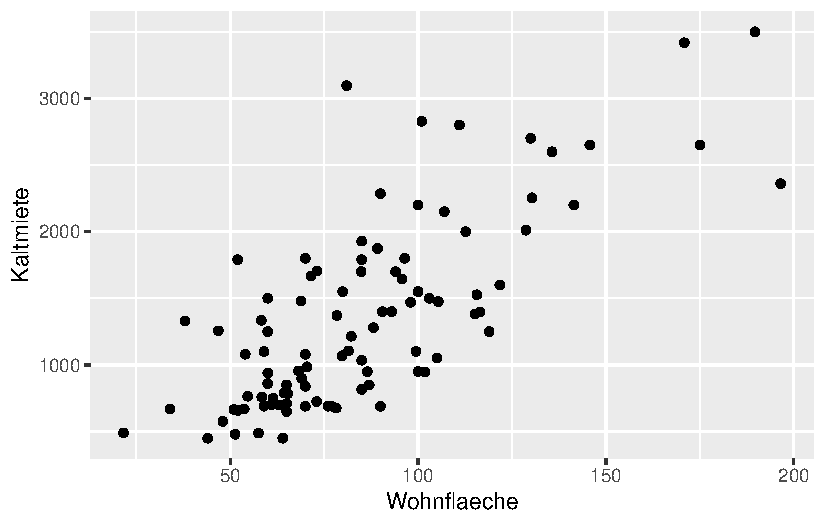
\includegraphics{Mietmodellierung_files/figure-pdf/unnamed-chunk-6-1.pdf}

}

\end{figure}

Grundsätzlich lässt sich ein positiver Zusammenhang zwischen
\texttt{Kaltmiete} und \texttt{Wohnflaeche} erkennen, wobei die Streuung
der Kaltmiete mit zunehmender Wohnfläche zunimmt. Nun muss dieses
Diagramm jedoch um die Information des Ortes erweitert werden, um eine
genauere Aussage treffen zu können. Dafür wird der Code um den Zusatz
\texttt{color\ =\ \textasciitilde{}\ Ort} erweitert:

\begin{Shaded}
\begin{Highlighting}[]
\FunctionTok{gf\_point}\NormalTok{(Kaltmiete }\SpecialCharTok{\textasciitilde{}}\NormalTok{ Wohnflaeche, }\AttributeTok{data =}\NormalTok{ mieten, }\AttributeTok{color =} \SpecialCharTok{\textasciitilde{}}\NormalTok{ Ort)}
\end{Highlighting}
\end{Shaded}

\begin{figure}[H]

{\centering 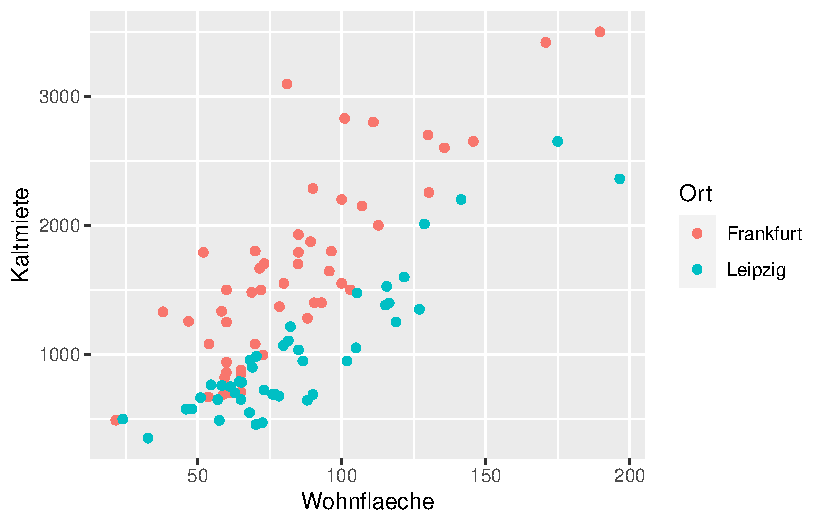
\includegraphics{Mietmodellierung_files/figure-pdf/unnamed-chunk-7-1.pdf}

}

\end{figure}

Hier lässt sich nun erkennen, dass die erfassten Mieten im Datensatz in
Frankfurt tendenziell höher sind, als in Leipzig. Bei vergleichbarer
Wohnfläche liegen die gefärbten Punkte für Frankfurt stets über den
Punkten von Leipzig. Um den Eindruck der Mietunterschiede zu festigen,
kann ein Boxplot verwendet werden.

\begin{Shaded}
\begin{Highlighting}[]
\FunctionTok{gf\_boxplot}\NormalTok{(Kaltmiete }\SpecialCharTok{\textasciitilde{}}\NormalTok{ Ort, }\AttributeTok{data =}\NormalTok{ mieten)}
\end{Highlighting}
\end{Shaded}

\begin{figure}[H]

{\centering 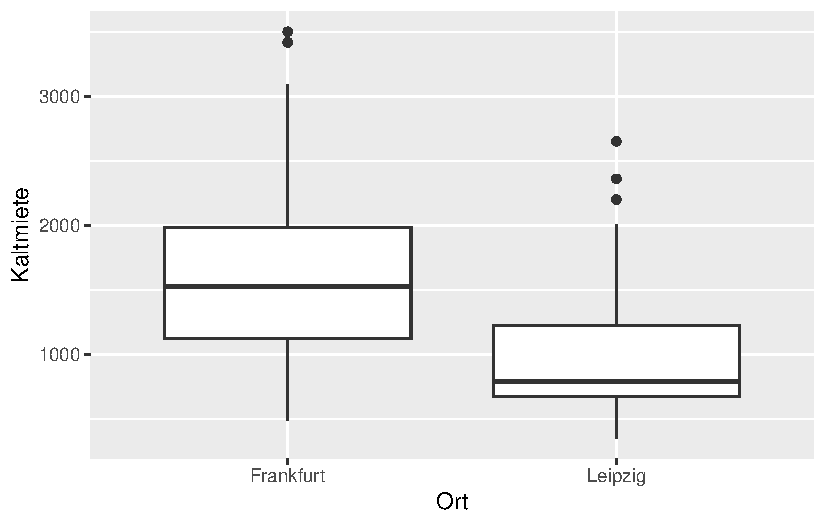
\includegraphics{Mietmodellierung_files/figure-pdf/unnamed-chunk-8-1.pdf}

}

\end{figure}

Das Boxplot zeigt, dass der Median für die Kaltmiete in Frankfurt
deutlich über dem Median von Leipzig liegt. Zudem ist der 1,5-fache
Interquartilsabstand bei Frankfurt größer als bei Leipzig, und die
Whisker sind bei Frankfurt ebenfalls länger. Für Leipzig gibt es jedoch
mehr Ausreißer, nämlich 4, verglichen mit den 2 Ausreißern von
Frankfurt. Mithilfe der Funktion \texttt{mean} kann der Mittelwerte der
Mieten in beiden Städten betrachtet werden.

\begin{Shaded}
\begin{Highlighting}[]
\FunctionTok{mean}\NormalTok{(}\SpecialCharTok{\textasciitilde{}}\NormalTok{ Kaltmiete, }\AttributeTok{data =}\NormalTok{ miete\_ffm)}
\end{Highlighting}
\end{Shaded}

\begin{verbatim}
[1] 1652.821
\end{verbatim}

\begin{Shaded}
\begin{Highlighting}[]
\FunctionTok{mean}\NormalTok{(}\SpecialCharTok{\textasciitilde{}}\NormalTok{ Kaltmiete, }\AttributeTok{data =}\NormalTok{ miete\_lpz)}
\end{Highlighting}
\end{Shaded}

\begin{verbatim}
[1] 1019.461
\end{verbatim}

Der Mittelwert für die Kaltmiete liegt in Frankfurt bei 1.652,82€ und
damit mehr als 600€ über dem Kaltmietendurchschnitt von Leipzig
(1.011,64€).

Es sollen nun auch die weiteren Variablen untersucht werden, angefangen
mit der Variablen \texttt{Heizung}. Um die verschiedenen Ausprägungen zu
vergleichen und ihre absolute Häufigkeit darzustellen, eignet sich ein
Säulendiagramm:

\begin{Shaded}
\begin{Highlighting}[]
\FunctionTok{gf\_bar}\NormalTok{( }\SpecialCharTok{\textasciitilde{}}\NormalTok{ Heizung, }\AttributeTok{data =}\NormalTok{ mieten, }\AttributeTok{fill =} \SpecialCharTok{\textasciitilde{}}\NormalTok{ Ort, }\AttributeTok{position =} \FunctionTok{position\_dodge}\NormalTok{()) }\SpecialCharTok{+} \FunctionTok{theme}\NormalTok{(}\AttributeTok{axis.text.x =} \FunctionTok{element\_text}\NormalTok{(}\AttributeTok{angle =} \DecValTok{90}\NormalTok{))}
\end{Highlighting}
\end{Shaded}

\begin{figure}[H]

{\centering 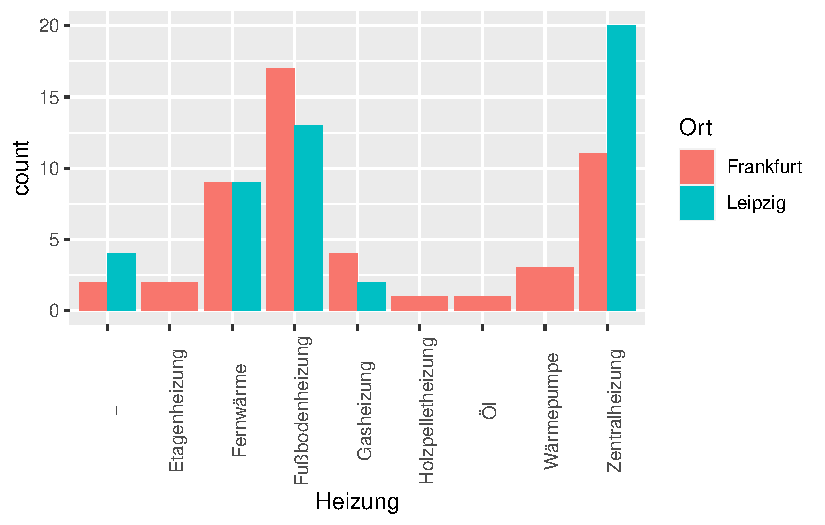
\includegraphics{Mietmodellierung_files/figure-pdf/unnamed-chunk-10-1.pdf}

}

\end{figure}

Das Säulendiagramm zeigt, dass die Fußbodenheizung in Frankfurt am
weitesten verbreitet ist, gefolgt von der Zentralheizung und der
Fernwärme. In Leipzig ist die Zentralheizung am weitesten verbreitet,
gefolgt von der Fußbodenheizung und der Fernwärme. In einigen
Beobachtungen und häufiger in Leipzig als in Frankfurt, wurde der
Heizungstyp nicht angegeben.

Bei der Variablen \texttt{Baujahr} handelt es sich hier um eine diskrete
Variable. Aufgrund der Vielzahl an verschiedenen Jahren im Datensatz
eignet sich jedoch die Verwendung des tatsächlichen Baujahres nicht, da
die Darstellungen sonst sehr unübersichtlich werden. Stattdessen soll
eine Klassifizierung in ``alt - mittel - neu'' vorgenommen werden, um
die Baujahre zusammenzufassen.

\begin{Shaded}
\begin{Highlighting}[]
\NormalTok{mieten }\OtherTok{\textless{}{-}}\NormalTok{ mieten }\SpecialCharTok{\%\textgreater{}\%}
  \FunctionTok{mutate}\NormalTok{(}\AttributeTok{Baujahrgruppe =} \FunctionTok{case\_when}\NormalTok{(}
    \FunctionTok{is.na}\NormalTok{(Baujahr) }\SpecialCharTok{\textasciitilde{}} \StringTok{"NA"}\NormalTok{,}
    \FunctionTok{as.integer}\NormalTok{(Baujahr) }\SpecialCharTok{\textless{}} \DecValTok{1970} \SpecialCharTok{\textasciitilde{}} \StringTok{"alt"}\NormalTok{,}
    \FunctionTok{between}\NormalTok{(}\FunctionTok{as.integer}\NormalTok{(Baujahr), }\DecValTok{1970}\NormalTok{, }\DecValTok{2000}\NormalTok{) }\SpecialCharTok{\textasciitilde{}} \StringTok{"mittel"}\NormalTok{,}
    \ConstantTok{TRUE} \SpecialCharTok{\textasciitilde{}} \StringTok{"neu"}
\NormalTok{  ))}

\FunctionTok{gf\_bar}\NormalTok{( }\SpecialCharTok{\textasciitilde{}}\NormalTok{ Baujahrgruppe, }\AttributeTok{data =}\NormalTok{ mieten, }\AttributeTok{fill =} \SpecialCharTok{\textasciitilde{}}\NormalTok{ Ort, }\AttributeTok{position =} \FunctionTok{position\_dodge}\NormalTok{())}
\end{Highlighting}
\end{Shaded}

\begin{figure}[H]

{\centering 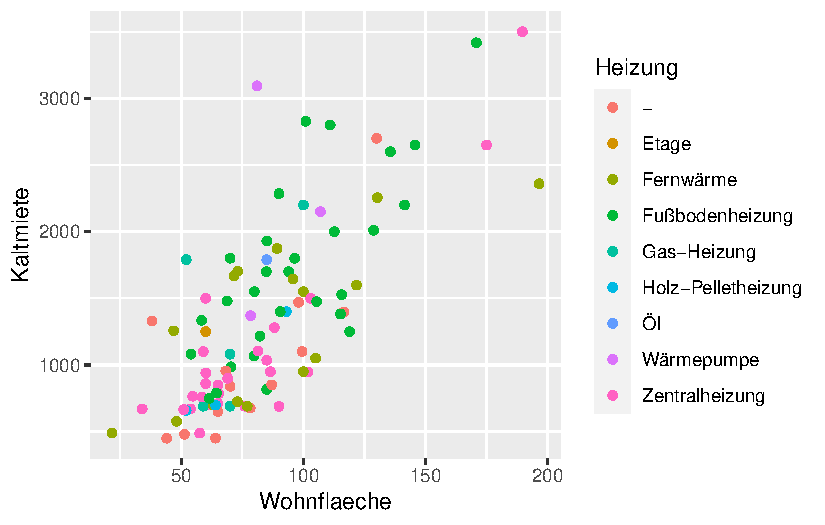
\includegraphics{Mietmodellierung_files/figure-pdf/unnamed-chunk-11-1.pdf}

}

\end{figure}

Im Säulendiagramm ist erkennbar, dass die meisten Beobachtungen in
Frankfurt in die Kategorie \texttt{neu} (Baujahr \textgreater{} 2000)
fallen, gefolgt von \texttt{alt} (Baujahr \textless{} 1970) und
\texttt{mittel}. In Leipzig dominieren die Beobachtungen mit
\texttt{alt}, dann kommen \texttt{neu}e Baujahre. Es treten in beiden
Städten nur wenige Beobachtungen mit Baujahren zwischen 1970 und 2000
auf.

\hypertarget{parkplatz}{%
\subsection{Parkplatz}\label{parkplatz}}

\begin{Shaded}
\begin{Highlighting}[]
\FunctionTok{gf\_boxplot}\NormalTok{(Kaltmiete }\SpecialCharTok{\textasciitilde{}}\NormalTok{ Parkplatz, }\AttributeTok{data =}\NormalTok{ mieten, }\AttributeTok{color =} \SpecialCharTok{\textasciitilde{}}\NormalTok{ Ort)}
\end{Highlighting}
\end{Shaded}

\begin{figure}[H]

{\centering 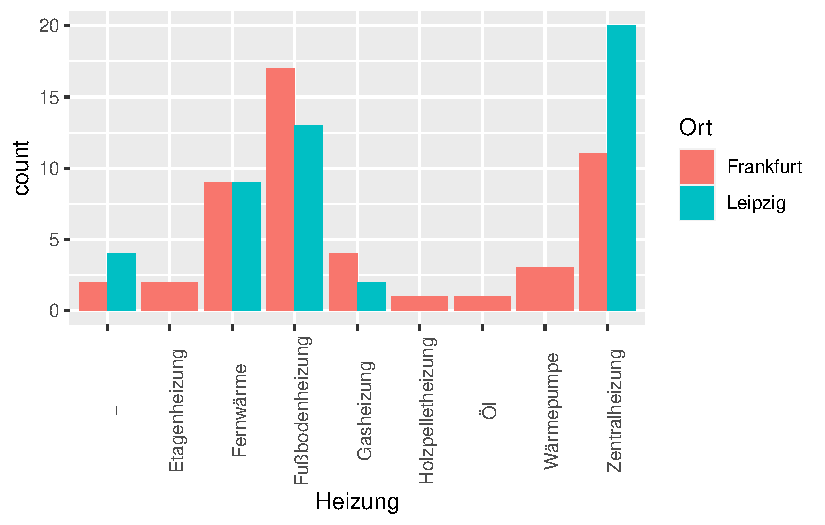
\includegraphics{Mietmodellierung_files/figure-pdf/unnamed-chunk-12-1.pdf}

}

\end{figure}

\begin{Shaded}
\begin{Highlighting}[]
\FunctionTok{tally}\NormalTok{(Ort }\SpecialCharTok{\textasciitilde{}}\NormalTok{ Parkplatz, }\AttributeTok{data =}\NormalTok{ mieten)}
\end{Highlighting}
\end{Shaded}

\begin{verbatim}
           Parkplatz
Ort         ja nein
  Frankfurt 26   24
  Leipzig   17   31
\end{verbatim}

Klare Tendenz in beiden Städten Wohnungen mit Parkplatz sind im Schnitt
teurer ? Parkplatz in der Kaltmiete enthalten? ? Eventuell teurere
Wohnung hat eher eine Tiefgarage oder einen sonstigen Stellplatz auf dem
Grundstück?

\hypertarget{balkon}{%
\subsection{Balkon}\label{balkon}}

\begin{Shaded}
\begin{Highlighting}[]
\FunctionTok{gf\_boxplot}\NormalTok{(Kaltmiete }\SpecialCharTok{\textasciitilde{}}\NormalTok{ Balkon, }\AttributeTok{data =}\NormalTok{ mieten, }\AttributeTok{color =} \SpecialCharTok{\textasciitilde{}}\NormalTok{ Ort)}
\end{Highlighting}
\end{Shaded}

\begin{figure}[H]

{\centering 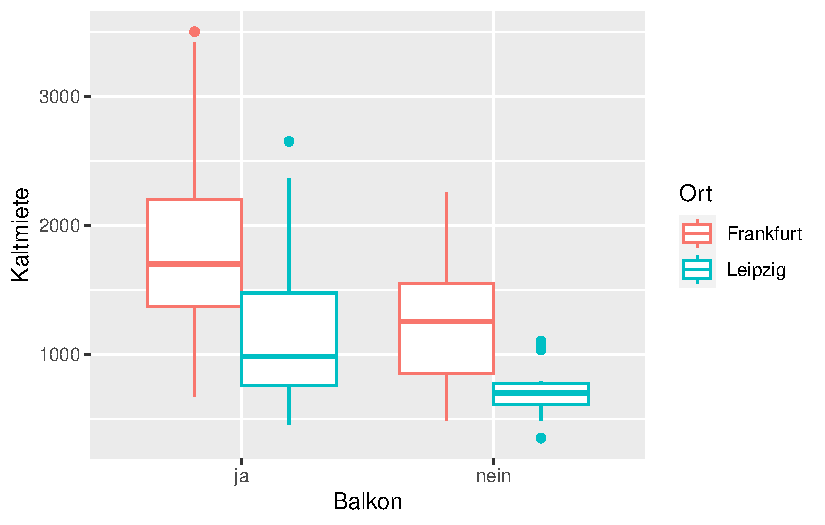
\includegraphics{Mietmodellierung_files/figure-pdf/unnamed-chunk-13-1.pdf}

}

\end{figure}

\begin{Shaded}
\begin{Highlighting}[]
\FunctionTok{gf\_boxplot}\NormalTok{(ppqm }\SpecialCharTok{\textasciitilde{}}\NormalTok{ Balkon, }\AttributeTok{data =}\NormalTok{ mieten, }\AttributeTok{color =} \SpecialCharTok{\textasciitilde{}}\NormalTok{ Ort)}
\end{Highlighting}
\end{Shaded}

\begin{figure}[H]

{\centering 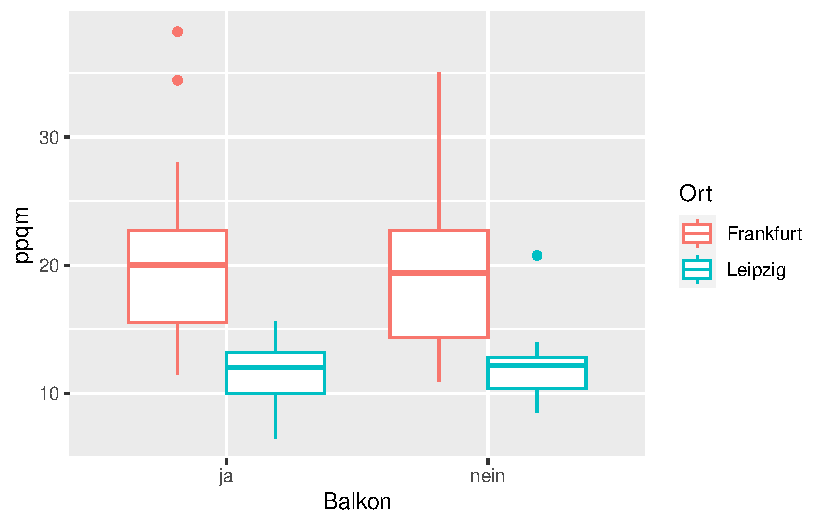
\includegraphics{Mietmodellierung_files/figure-pdf/unnamed-chunk-13-2.pdf}

}

\end{figure}

\begin{Shaded}
\begin{Highlighting}[]
\FunctionTok{tally}\NormalTok{(Ort }\SpecialCharTok{\textasciitilde{}}\NormalTok{ Balkon, }\AttributeTok{data =}\NormalTok{ mieten)}
\end{Highlighting}
\end{Shaded}

\begin{verbatim}
           Balkon
Ort         ja nein
  Frankfurt 37   13
  Leipzig   29   19
\end{verbatim}

Erstes Boxplot zeigt Wohnung mit Balkon sind meist teurer Da der Balkon
auch zu 25\% in die gesamte Wohnflaeche eingerechnet ist, wird im
zweiten Boxplot auch der Quadratmeterpreis betrachtet. Hier ist auch ein
Zusammenhang zwischen Balkon ``Ja'' und einen höheren Kaltmiete zu
erkennen. ?Interpretation: Balkon steigert Kaltmiete unabhängig von der
Wohnfläche. Interessant wäre zusätzlich eine Analyse, wenn Wohnfläcche
um die Fläche des Balkons bereinigt wäre.

\hypertarget{zimmer}{%
\subsection{Zimmer}\label{zimmer}}

\begin{Shaded}
\begin{Highlighting}[]
\FunctionTok{gf\_point}\NormalTok{(Kaltmiete }\SpecialCharTok{\textasciitilde{}}\NormalTok{ Zimmer, }\AttributeTok{data =}\NormalTok{ mieten, }\AttributeTok{color =} \SpecialCharTok{\textasciitilde{}}\NormalTok{ Ort)}
\end{Highlighting}
\end{Shaded}

\begin{figure}[H]

{\centering 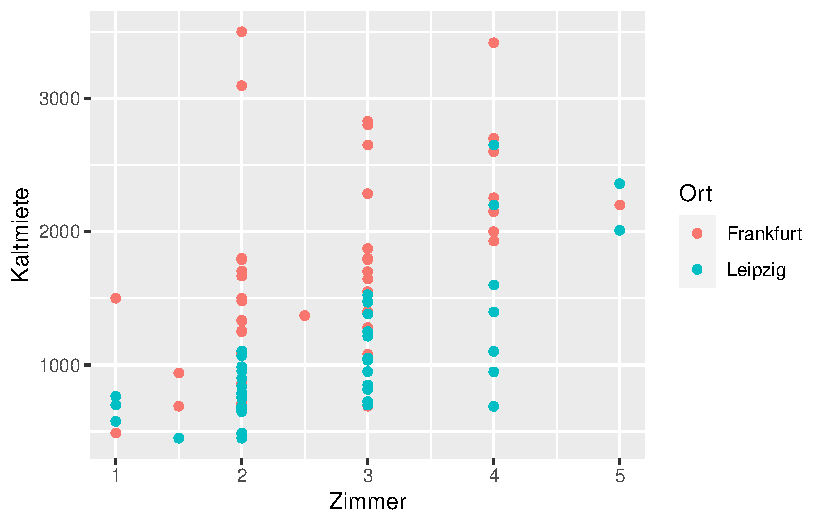
\includegraphics{Mietmodellierung_files/figure-pdf/unnamed-chunk-14-1.pdf}

}

\end{figure}

\begin{Shaded}
\begin{Highlighting}[]
\FunctionTok{gf\_point}\NormalTok{(Wohnflaeche }\SpecialCharTok{\textasciitilde{}}\NormalTok{ Zimmer, }\AttributeTok{data =}\NormalTok{ mieten, }\AttributeTok{color =} \SpecialCharTok{\textasciitilde{}}\NormalTok{ Ort)}
\end{Highlighting}
\end{Shaded}

\begin{figure}[H]

{\centering 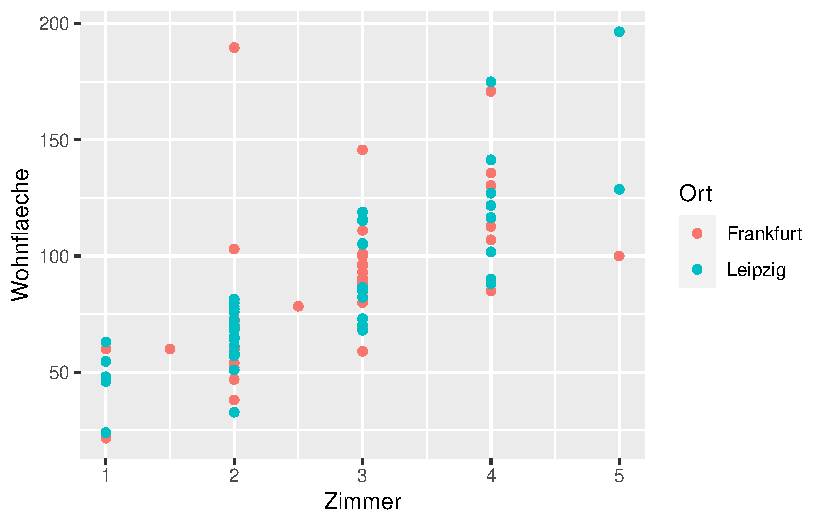
\includegraphics{Mietmodellierung_files/figure-pdf/unnamed-chunk-14-2.pdf}

}

\end{figure}

\begin{Shaded}
\begin{Highlighting}[]
\FunctionTok{gf\_point}\NormalTok{(ppqm }\SpecialCharTok{\textasciitilde{}}\NormalTok{ Zimmer, }\AttributeTok{data =}\NormalTok{ mieten, }\AttributeTok{color =} \SpecialCharTok{\textasciitilde{}}\NormalTok{ Ort)}
\end{Highlighting}
\end{Shaded}

\begin{figure}[H]

{\centering 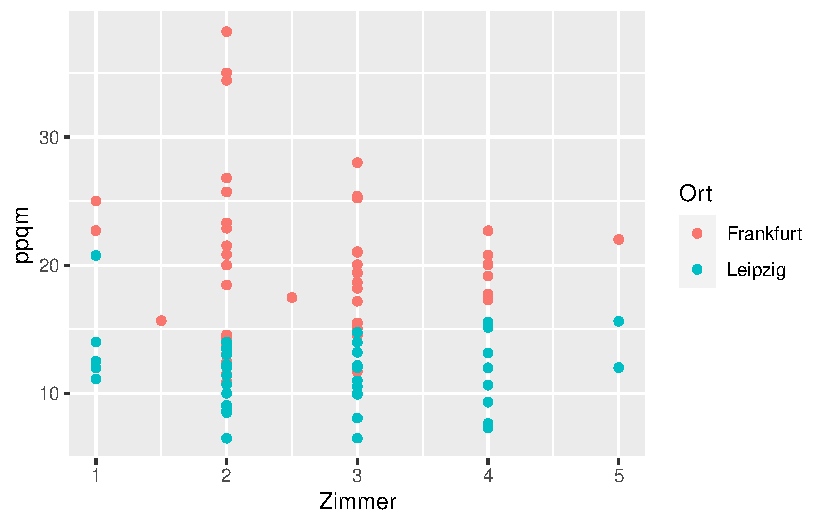
\includegraphics{Mietmodellierung_files/figure-pdf/unnamed-chunk-14-3.pdf}

}

\end{figure}

Insgesamt ist zu erkennen, dass die Variable Zimmer einen Einfluss auf
die Wohnfläche hat. Der Quadratmeterpreis ist bei mehr Zimmern nicht
höher.

\hypertarget{etage}{%
\subsection{Etage}\label{etage}}

\begin{Shaded}
\begin{Highlighting}[]
\FunctionTok{gf\_boxplot}\NormalTok{(Kaltmiete }\SpecialCharTok{\textasciitilde{}}\NormalTok{ Etage, }\AttributeTok{data =}\NormalTok{ mieten)}
\end{Highlighting}
\end{Shaded}

\begin{verbatim}
Warning: Continuous x aesthetic
i did you forget `aes(group = ...)`?
\end{verbatim}

\begin{figure}[H]

{\centering 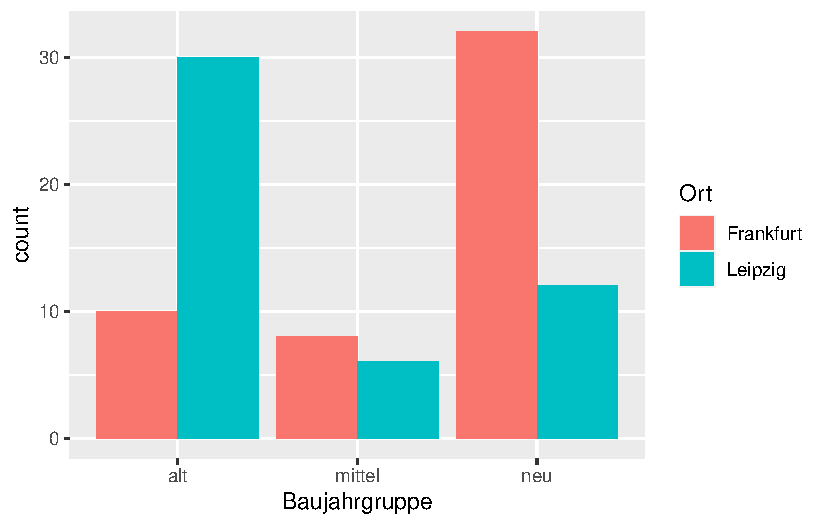
\includegraphics{Mietmodellierung_files/figure-pdf/unnamed-chunk-15-1.pdf}

}

\end{figure}

Schlecht bis gar nicht beschreibbar/interpretierbar

\hypertarget{modellierung}{%
\section{Modellierung}\label{modellierung}}

Aus den zahlreichen Diagrammen des vorherigen Abschnitts der
explorativen Datenanalyse konnten sich bereits diverse Zusammenhänge
erkennen lassen. Dieser letzte Teil der Untersuchung der gegebenen Daten
beschäftigt sich abschließend mit der Modellierung der Kaltmiete unter
Verwendung der zur Verfügung stehenden Variablen wie der Wohnfläche, der
Art der Heizung oder dem Vorhandensein eines Balkons. Ziel ist hierbei
die Erstellung eines Modells, durch das die Variable \texttt{Kaltmiete}
bestmöglich erklärt werden kann.

\hypertarget{modellierung-uxfcber-durchschnittsquadratmeterpreis}{%
\subsection{Modellierung über
Durchschnittsquadratmeterpreis}\label{modellierung-uxfcber-durchschnittsquadratmeterpreis}}

Das erste Diagramm der explorativen Datenanalyse, in dem die
\texttt{Kaltmiete} der Inserate zusammen mit deren \texttt{Wohnfläche}
im Streudiagramm dargestellt wurden, lässt einen positiven Zusammenhang
der \texttt{Kaltmiete} zur \texttt{Wohnfläche} vermuten. In einem ersten
einfachen Modell, mit dem dieser Zusammenhang modelliert werden soll,
kann aus den Daten beispielsweise der Durchschnitt des
Quadratmeterpreises berechnet werden.

\begin{Shaded}
\begin{Highlighting}[]
\NormalTok{sum\_wohnflaeche }\OtherTok{\textless{}{-}} \FunctionTok{sum}\NormalTok{(}\SpecialCharTok{\textasciitilde{}}\NormalTok{ Wohnflaeche, }\AttributeTok{data =}\NormalTok{ mieten)}
\NormalTok{sum\_kaltmiete }\OtherTok{\textless{}{-}} \FunctionTok{sum}\NormalTok{(}\SpecialCharTok{\textasciitilde{}}\NormalTok{ Kaltmiete, }\AttributeTok{data =}\NormalTok{ mieten)}
\NormalTok{price\_per\_squaremeter }\OtherTok{\textless{}{-}}\NormalTok{ sum\_kaltmiete }\SpecialCharTok{/}\NormalTok{ sum\_wohnflaeche}
\end{Highlighting}
\end{Shaded}

Damit ergibt sich als ersten einfaches Modell für die \texttt{Kaltmiete}
unter Verwendung der \texttt{Wohnfläche} als unabhängige Variable
folgende Gleichung:

\[ Kaltmiete = Wohnfläche \cdot 15.76 € \] Wir betrachten das Modell,
indem die berechnete Gerade in das Streudiagramm der explorativen
Datenanalyse eingezeichnet wird:

\begin{Shaded}
\begin{Highlighting}[]
\NormalTok{pps\_x }\OtherTok{=} \FunctionTok{c}\NormalTok{(}\DecValTok{0}\NormalTok{, }\DecValTok{200}\NormalTok{)}
\NormalTok{pps\_y }\OtherTok{=} \FunctionTok{c}\NormalTok{(}\DecValTok{0}\NormalTok{, price\_per\_squaremeter }\SpecialCharTok{*} \DecValTok{200}\NormalTok{)}
\FunctionTok{gf\_line}\NormalTok{(pps\_y }\SpecialCharTok{\textasciitilde{}}\NormalTok{ pps\_x, }\AttributeTok{color =} \StringTok{"blue"}\NormalTok{) }\SpecialCharTok{|\textgreater{}} 
  \FunctionTok{gf\_point}\NormalTok{(Kaltmiete }\SpecialCharTok{\textasciitilde{}}\NormalTok{ Wohnflaeche, }\AttributeTok{data =}\NormalTok{ mieten, }\AttributeTok{color =} \SpecialCharTok{\textasciitilde{}}\NormalTok{ Ort) }\SpecialCharTok{|\textgreater{}} 
  \FunctionTok{gf\_labs}\NormalTok{(}\AttributeTok{x =} \StringTok{"Wohnfläche in Quadratmeter"}\NormalTok{, }
          \AttributeTok{y =} \StringTok{"Mietpreis in Euro"}\NormalTok{, }
          \AttributeTok{title =} \StringTok{"Modellierung über Durchschnittspreis"}\NormalTok{)}
\end{Highlighting}
\end{Shaded}

\begin{figure}[H]

{\centering 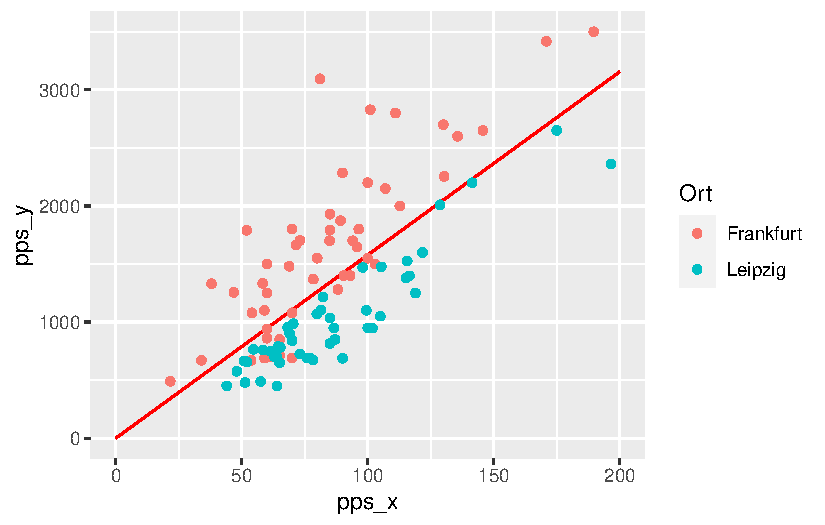
\includegraphics{Mietmodellierung_files/figure-pdf/unnamed-chunk-17-1.pdf}

}

\end{figure}

Dazu kann noch der Korrelationskoeffizient bestimmt werden.

\begin{Shaded}
\begin{Highlighting}[]
\NormalTok{cor\_miete\_flaeche }\OtherTok{=} \FunctionTok{cor}\NormalTok{(Wohnflaeche }\SpecialCharTok{\textasciitilde{}}\NormalTok{ Kaltmiete, }\AttributeTok{data =}\NormalTok{ mieten)}
\end{Highlighting}
\end{Shaded}

Dabei wird festgestellt, dass die \texttt{Kaltmiete} zu 74.54\% mit der
Wohnfläche korreliert. Das Modell kann demnach bereits für einen groben
Richtwert verwendet werden. Ziel ist jedoch eine noch genauere
Modellierung der Kaltmiete unter Berücksichtigung der weiteren Daten.

\hypertarget{modellierung-uxfcber-die-lineare-regression}{%
\subsection{Modellierung über die lineare
Regression}\label{modellierung-uxfcber-die-lineare-regression}}

Um die weiteren Variablen miteinzubeziehen, verwenden wir die lineare
Regression, die mit der \texttt{lm()}-Funktion auf die Daten angewendet
werden kann.

\hypertarget{wohnflaeche}{%
\subsubsection{Wohnflaeche}\label{wohnflaeche}}

Wir starten zunächst erneut mit der \texttt{Kaltmiete} und der jeweils
dazugehörigen \texttt{Wohnflaeche}.

\begin{Shaded}
\begin{Highlighting}[]
\NormalTok{km.lm1 }\OtherTok{\textless{}{-}} \FunctionTok{lm}\NormalTok{(Kaltmiete }\SpecialCharTok{\textasciitilde{}}\NormalTok{ Wohnflaeche, }\AttributeTok{data =}\NormalTok{ mieten)}
\FunctionTok{summary}\NormalTok{(km.lm1)}
\end{Highlighting}
\end{Shaded}

\begin{verbatim}

Call:
lm(formula = Kaltmiete ~ Wohnflaeche, data = mieten)

Residuals:
   Min     1Q Median     3Q    Max 
-742.4 -295.9 -123.8  345.7 1817.6 

Coefficients:
            Estimate Std. Error t value Pr(>|t|)    
(Intercept)   24.403    129.718   0.188    0.851    
Wohnflaeche   15.469      1.412  10.956   <2e-16 ***
---
Signif. codes:  0 '***' 0.001 '**' 0.01 '*' 0.05 '.' 0.1 ' ' 1

Residual standard error: 479.8 on 96 degrees of freedom
Multiple R-squared:  0.5556,    Adjusted R-squared:  0.551 
F-statistic:   120 on 1 and 96 DF,  p-value: < 2.2e-16
\end{verbatim}

Mit einem Bestimmtheitsmaß von \(R^2 = 0.55\), haben wir mit der
linearen Regression allein unter Verwendung der \texttt{Wonflaeche} noch
kein gutes Modell erzeugt.

\hypertarget{ort}{%
\subsubsection{Ort}\label{ort}}

Da zu Beginn der explorativen Datenanalyse festgestellt wurde, dass sich
die Kaltmieten zwischen den beiden Orten Frankfurt am Main und Leipzig
unter sonst gleichen Bedingungen bereits stark unterscheidet, soll diese
zuerst in die Modellierung miteinbezogen werden.

\begin{Shaded}
\begin{Highlighting}[]
\NormalTok{km.lm2 }\OtherTok{\textless{}{-}} \FunctionTok{lm}\NormalTok{(Kaltmiete }\SpecialCharTok{\textasciitilde{}}\NormalTok{ Wohnflaeche }\SpecialCharTok{+}\NormalTok{ Ort, }\AttributeTok{data =}\NormalTok{ mieten)}
\FunctionTok{summary}\NormalTok{(km.lm2)}
\end{Highlighting}
\end{Shaded}

\begin{verbatim}

Call:
lm(formula = Kaltmiete ~ Wohnflaeche + Ort, data = mieten)

Residuals:
    Min      1Q  Median      3Q     Max 
-640.01 -279.07   36.35  188.68 1492.90 

Coefficients:
            Estimate Std. Error t value Pr(>|t|)    
(Intercept)  325.853     98.305   3.315   0.0013 ** 
Wohnflaeche   15.756      1.014  15.540  < 2e-16 ***
OrtLeipzig  -665.433     69.627  -9.557 1.46e-15 ***
---
Signif. codes:  0 '***' 0.001 '**' 0.01 '*' 0.05 '.' 0.1 ' ' 1

Residual standard error: 344.4 on 95 degrees of freedom
Multiple R-squared:  0.7734,    Adjusted R-squared:  0.7687 
F-statistic: 162.2 on 2 and 95 DF,  p-value: < 2.2e-16
\end{verbatim}

\begin{Shaded}
\begin{Highlighting}[]
\NormalTok{km.lm2.coef }\OtherTok{\textless{}{-}} \FunctionTok{coef}\NormalTok{(km.lm2)}
\FunctionTok{print}\NormalTok{(km.lm2.coef)}
\end{Highlighting}
\end{Shaded}

\begin{verbatim}
(Intercept) Wohnflaeche  OrtLeipzig 
   325.8526     15.7562   -665.4331 
\end{verbatim}

it dem Miteinbeziehen der Indekatorvariable \(x2\) beziehungsweise der
kategorialen Variable des Ortes erhalten wir ein Bestimmtheitsmaß von
\(R^2 = 0.77\). Die Variation des Mietpreises kann also zu \(78\)\%
durch den Mietpreis und dem Ort erklärt werden. An der Zusammenfassung
der Ergebnisse lässt sich außerdem ablesen, dass in Leipzig die
Kaltmiete im Mittelwert 655,13€ billiger als in Leipzig ist. Das Modell
lässt sich nun wie folgt darstellen:

\[ 
\hat{y}_i = 
325.85 
+ x1_i \cdot 
15.76
-665.43 \cdot 
\begin{cases} 
\text{1}: & \text{ $x2_i = Leipzig$}\\
\text{0}: & \text{ $x2_i = Frankfurt$}
\end{cases} 
\]

Wobei \(x1_i\) die \texttt{Wohnflaeche} und \(x2_i\) entsprechend den
\texttt{Wohnort} darstellt.

Entsprechend dem berechneten P-Wert von \(3.68 \cdot 10^(-16)\) kann das
Ergebnis in Bezug auf den Wohnort unter Verwendung eines
Signifikanzniveaus von \(5\%\) als statistisch signifikant bezeichnet
werden. Die \(H_0\)-Hypothese \(\mu_{Frankfurt} = \mu_{Leipzig}\) kann
somit verworfen werden.

Grafisch erhalten wir dadurch die zwei Geraden, abhängig des Ortes:

\begin{Shaded}
\begin{Highlighting}[]
\NormalTok{frankfurt.x }\OtherTok{=} \FunctionTok{c}\NormalTok{(}\DecValTok{0}\NormalTok{, }\DecValTok{200}\NormalTok{)}
\NormalTok{frankfurt.y }\OtherTok{=} \FunctionTok{c}\NormalTok{(km.lm2.coef[}\DecValTok{1}\NormalTok{] }\SpecialCharTok{+}\NormalTok{ km.lm2.coef[}\DecValTok{2}\NormalTok{] }\SpecialCharTok{*} \DecValTok{0} \SpecialCharTok{+}\NormalTok{ km.lm2.coef[}\DecValTok{3}\NormalTok{] }\SpecialCharTok{*} \DecValTok{0}\NormalTok{, km.lm2.coef[}\DecValTok{1}\NormalTok{] }\SpecialCharTok{+}\NormalTok{ km.lm2.coef[}\DecValTok{2}\NormalTok{] }\SpecialCharTok{*} \DecValTok{200} \SpecialCharTok{+}\NormalTok{ km.lm2.coef[}\DecValTok{3}\NormalTok{] }\SpecialCharTok{*} \DecValTok{0}\NormalTok{ )}
\NormalTok{leipzig.x }\OtherTok{=} \FunctionTok{c}\NormalTok{(}\DecValTok{0}\NormalTok{, }\DecValTok{200}\NormalTok{)}
\NormalTok{leipzig.y }\OtherTok{=} \FunctionTok{c}\NormalTok{(km.lm2.coef[}\DecValTok{1}\NormalTok{] }\SpecialCharTok{+}\NormalTok{ km.lm2.coef[}\DecValTok{2}\NormalTok{] }\SpecialCharTok{*} \DecValTok{0} \SpecialCharTok{+}\NormalTok{ km.lm2.coef[}\DecValTok{3}\NormalTok{] }\SpecialCharTok{*} \DecValTok{1}\NormalTok{, km.lm2.coef[}\DecValTok{1}\NormalTok{] }\SpecialCharTok{+}\NormalTok{ km.lm2.coef[}\DecValTok{2}\NormalTok{] }\SpecialCharTok{*} \DecValTok{200} \SpecialCharTok{+}\NormalTok{ km.lm2.coef[}\DecValTok{3}\NormalTok{] }\SpecialCharTok{*} \DecValTok{1}\NormalTok{ )}
\NormalTok{pps\_y }\OtherTok{=} \FunctionTok{c}\NormalTok{(}\DecValTok{0}\NormalTok{, price\_per\_squaremeter }\SpecialCharTok{*} \DecValTok{200}\NormalTok{)}
\FunctionTok{gf\_line}\NormalTok{(frankfurt.y }\SpecialCharTok{\textasciitilde{}}\NormalTok{ frankfurt.x, }\AttributeTok{color =} \StringTok{"orange"}\NormalTok{) }\SpecialCharTok{|\textgreater{}} 
  \FunctionTok{gf\_line}\NormalTok{(leipzig.y }\SpecialCharTok{\textasciitilde{}}\NormalTok{ leipzig.x, }\AttributeTok{color =} \StringTok{"lightblue"}\NormalTok{) }\SpecialCharTok{|\textgreater{}}
  \FunctionTok{gf\_point}\NormalTok{(Kaltmiete }\SpecialCharTok{\textasciitilde{}}\NormalTok{ Wohnflaeche, }\AttributeTok{data =}\NormalTok{ mieten, }\AttributeTok{color =} \SpecialCharTok{\textasciitilde{}}\NormalTok{ Ort)}
\end{Highlighting}
\end{Shaded}

\begin{figure}[H]

{\centering 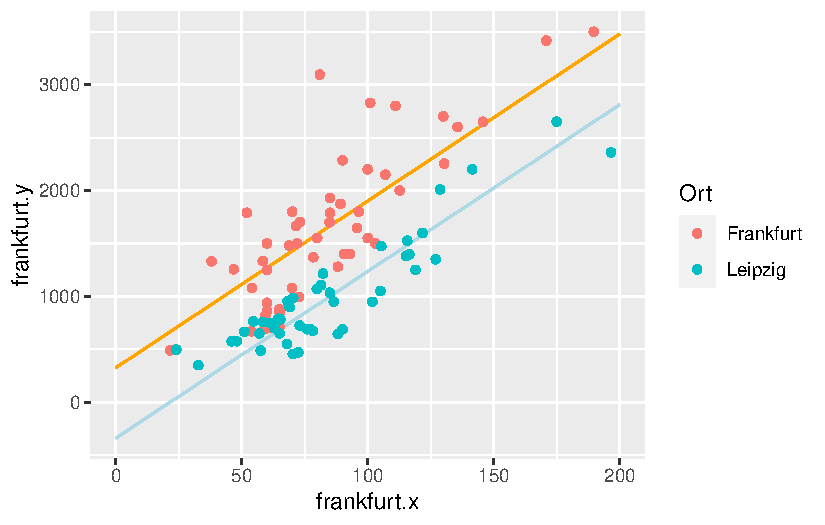
\includegraphics{Mietmodellierung_files/figure-pdf/unnamed-chunk-22-1.pdf}

}

\end{figure}

Sowohl grafisch als auch am Bestimmtheitsmaß ist bereits sichtbar, dass
die Modellierung über die Größe der Immobilien zusammen mit dem
jeweiligen Ort einen großen Teil des Mietpreises erklären kann.

\hypertarget{weitere-variablen}{%
\subsubsection{Weitere Variablen}\label{weitere-variablen}}

Zuletzt werden die weiteren Variablen in die lineare Regression
miteinbezogen und das daraus entstehende Modell betrachtet und
interpretiert. Wir verwenden nun zusätzlich die Informationen bezüglich
des \texttt{Parkplatzes}, der Anzahl der Zimmer, des \texttt{Baujahres},
das Vorhandensein eines Balkons und der \texttt{Etage}.

\begin{Shaded}
\begin{Highlighting}[]
\NormalTok{km.lm3 }\OtherTok{\textless{}{-}} \FunctionTok{lm}\NormalTok{(Kaltmiete }\SpecialCharTok{\textasciitilde{}}\NormalTok{ Wohnflaeche }\SpecialCharTok{+}\NormalTok{ Ort }\SpecialCharTok{+}\NormalTok{ Parkplatz }\SpecialCharTok{+}\NormalTok{ Balkon }\SpecialCharTok{+}\NormalTok{ Baujahr }\SpecialCharTok{+}\NormalTok{ Etage }\SpecialCharTok{+}\NormalTok{ Zimmer }\SpecialCharTok{+}\NormalTok{ Heizung, }\AttributeTok{data =}\NormalTok{ mieten)}
\FunctionTok{summary}\NormalTok{(km.lm3)}
\end{Highlighting}
\end{Shaded}

\begin{verbatim}

Call:
lm(formula = Kaltmiete ~ Wohnflaeche + Ort + Parkplatz + Balkon + 
    Baujahr + Etage + Zimmer + Heizung, data = mieten)

Residuals:
    Min      1Q  Median      3Q     Max 
-461.26 -188.96  -42.04  160.67  766.81 

Coefficients:
                           Estimate Std. Error t value Pr(>|t|)    
(Intercept)              -3620.3704  1580.1647  -2.291  0.02452 *  
Wohnflaeche                 16.9243     1.3807  12.258  < 2e-16 ***
OrtLeipzig                -466.3345    70.2276  -6.640 3.17e-09 ***
Parkplatznein             -149.0587    69.5677  -2.143  0.03511 *  
Balkonnein                  28.5883    69.1350   0.414  0.68031    
Baujahr                      2.0359     0.7735   2.632  0.01014 *  
Etage                       23.3075     6.7295   3.463  0.00085 ***
Zimmer                     -71.6654    47.1581  -1.520  0.13244    
HeizungEtagenheizung         3.9650   242.2408   0.016  0.98698    
HeizungFernwärme          -176.2000   130.4222  -1.351  0.18041    
HeizungFußbodenheizung     -20.6200   126.5903  -0.163  0.87101    
HeizungGasheizung          176.2957   167.9711   1.050  0.29700    
HeizungHolzpelletheizung  -289.8749   303.4758  -0.955  0.34229    
HeizungÖl                   92.0784   304.4141   0.302  0.76305    
HeizungWärmepumpe          196.3236   210.3614   0.933  0.35342    
HeizungZentralheizung     -171.7000   125.3993  -1.369  0.17467    
---
Signif. codes:  0 '***' 0.001 '**' 0.01 '*' 0.05 '.' 0.1 ' ' 1

Residual standard error: 273.8 on 82 degrees of freedom
Multiple R-squared:  0.8764,    Adjusted R-squared:  0.8538 
F-statistic: 38.78 on 15 and 82 DF,  p-value: < 2.2e-16
\end{verbatim}

Zu sehen ist, dass wir unter dem Miteinbeziehen aller Informationen, die
zur Verfügung stehen, dennoch nur ein Bestimmtheitsmaß von \(R = 0.85\)
erreichen. Das bedeutet, dass trotz aller Daten, die Variation der
Mietpreise nur zu ca. \(85\%\) erklärt werden kann, was entsprechend
\(15\%\) unerklärt lässt.

Wie bereits in der vorherigen linearen Regression zu sehen war, hat
sowohl der Ort als auch die Wohnfläche einen starken Einfluss auf den
Wohnpreis. Beide Attribute sind unter einem Signifikanzniveau von
\(\alpha = 0.001\) statistisch signifkant. Dass der Ort und die Größe
der Wohnung einen erheblichen Einfluss auf den Mietpreis nehmen, ist
nicht weiter überraschend. Unter dem gleichen Signifikanzniveau
statistisch signifikant ist ebenso die Etage, in der die Wohnung liegt.
Wir sehen hier im Mittel einen Anstieg des Mietpreises um ca. \(23,00€\)
pro Etage. Begründen lässt sich dies eventuell durch die bessere
Aussicht in den oberen Etagen und die Wahrscheinlichkeiten auf
Wohnungstypen wie Penthäuser gesteigert ist.

Unter einem Signifikanzniveau von \(\alpha = 0.05\) statistisch relevant
ist sowohl das Vorhandensein eines Parkplatzes als auch das Baujahr. Ist
kein Parkplatz vorhanden, so ist der Mietpreis im Mittel ca. \(150,00€\)
billiger. Da Parkplätze insbesondere in Großstädten, aufgrund der
wenigen Parkmöglichkeiten, eine wichtige Rolle spielen ist verständlich.
Mit dem Baujahr steigt der Mietpreis im Mittel um ca. \(2,00€\). Neuere
Immobilien kommen in der Regel mit effizienteren Bauweisen, geringen
Energieverbräuchen und modernerem Aussehen und benötigen zumeist geringe
Wartungsarbeiten. Daher überrascht es nicht weiter, dass das Baujahr
einen Einfluss auf den Mietpreis nimmt.

Anhand der einzelnen P-Werte für die jeweiligen Attribute der Wohnungen
können wir außerdem ablesen, welche der Informationen für die
Modellierung des Mietpreises nicht signifikant ist. Dazu zählt zunächst
die Art der Heizung, von welcher keiner der aufgelisteten
Merkmalsausprägungen im Bereich des Signifikanzniveaus liegt. Dass die
Art der Heizung einen Einfluss auf den Mietpreis besitzt, kann durch die
uns zur Verfügung stehenden Daten also nicht bestätigt werden.

Ebenso zeigen die Daten keinen statistisch signifikanten Zusammenhang
zwischen der Anzahl der Zimmer und den Mietpreisen. Eine mögliche
Begründung ist, dass weniger die Aufteilung der Wohnung in \(n\)
verschiedene Zimmer, sondern die Größe der Wohnfläche für den Mietpreis
relevant ist. Beispielsweise kann sowohl eine besonders große Wohnung
als auch eine kleinere Wohnung aus insgesamt drei Zimmern bestehen. Der
Mietpreis wird bei der größeren Wohnung dennoch tendenziell größer sein,
wie die Daten bestätigen, da die Anzahl der Zimmer nichts über die Größe
der Wohnung aussagt.

Auch für das Vorhandensein eines Balkons lässt sich kein Einfluss auf
den Mietpreis feststellen. Mit einem P-Wert von \(p = 0.68\) ist hier
jegliches Signifikanzniveau überschritten. Begründet kann dies dadurch
sein, dass keine weiteren Informationen zu dem jeweiligen Balkon gegeben
ist. Wichtig könnte eventuell die Größe des Balkons, die Aussicht oder
weitere Faktoren sein, die hier nicht näher spezifiziert sind.

\begin{Shaded}
\begin{Highlighting}[]
\FunctionTok{confint}\NormalTok{(km.lm3)}
\end{Highlighting}
\end{Shaded}

\begin{verbatim}
                                 2.5 %      97.5 %
(Intercept)              -6763.8212789 -476.919434
Wohnflaeche                 14.1777598   19.670888
OrtLeipzig                -606.0396286 -326.629395
Parkplatznein             -287.4509890  -10.666461
Balkonnein                -108.9433026  166.119836
Baujahr                      0.4971043    3.574731
Etage                        9.9204314   36.694648
Zimmer                    -165.4778752   22.147140
HeizungEtagenheizung      -477.9291640  485.859142
HeizungFernwärme          -435.6513022   83.251224
HeizungFußbodenheizung    -272.4485677  231.208469
HeizungGasheizung         -157.8522989  510.443644
HeizungHolzpelletheizung  -893.5848651  313.835146
HeizungÖl                 -513.4982048  697.654927
HeizungWärmepumpe         -222.1521718  614.799343
HeizungZentralheizung     -421.1590358   77.759091
\end{verbatim}

Betrachten wir Abschließend die Konfidenzintervalle, so lässt sich
sagen, dass die Quadratmeteranzahl zu 95\% eine Auswirkung zwischen
\(14,18€\) und \(19,67€\) pro auf den Mietpreis in der Population hat.
Der Unterschied zwischen Frankfurt und Leipzig liegt mit gleicher
Wahrscheinlichkeit im Intervall von \(-606,04€\) und \(-326,63€\).

\hypertarget{zusammenfassung}{%
\section{Zusammenfassung}\label{zusammenfassung}}

Lorem ipsum dolor sit amet, consetetur sadipscing elitr, sed diam nonumy
eirmod tempor invidunt ut labore et dolore magna aliquyam erat, sed diam
voluptua. At vero eos et accusam et justo duo dolores et ea rebum. Stet
clita kasd gubergren, no sea takimata sanctus est Lorem ipsum dolor sit
amet. Lorem ipsum dolor sit amet, consetetur sadipscing elitr, sed diam
nonumy eirmod tempor invidunt ut labore et dolore magna aliquyam erat,
sed diam voluptua. At vero eos et accusam et justo duo dolores et ea
rebum. Stet clita kasd gubergren, no sea takimata sanctus est Lorem
ipsum dolor sit amet.

\begin{center}\rule{0.5\linewidth}{0.5pt}\end{center}

\hypertarget{quellen-und-hilfsmittel}{%
\section{Quellen und Hilfsmittel}\label{quellen-und-hilfsmittel}}

Führen Sie hier die verwendeten Hilfsmittel sowie die verwendete
Literatur auf.



\end{document}
